\section{Introduction}\label{sec:introduction}

Throughout the Army, Industrial Hygiene (IH) teams are responsible for inspection, environmental reconnaissance, and emergency response. Industrial hygiene is an integral part of installation force protection and is an important component of an installation’s toxic industrial chemical spill planned response. Current best practices for conducting the IH mission requires direct human exposure to these hazardous environments. Robotic systems offer the potential to remove humans from these dangerous situations while maintaining the reliability and accuracy of the response team. Applying robotic solutions to this domain also contribute to the Department of Defense (DoD) unmanned systems goals outlined in the Unmanned Systems Integrated Roadmap FY2011-2036 \cite{roadmap}. Furthermore, robotic IH solutions are a force multiplier because these systems can be sent into a hazardous environment, parked, and allowed to collect data autonomously. Additionally, using robotic platforms for the IH environment is faster and safer than equipping and decontaminating a human. Finally, if successful, this project has potential DoD-wide applications. 

\subsection{Trends}

Aging stocks of munitions and newly developed systems are creating larger quantities of dangerous materials that require monitoring and potentially, emergency response. In the current austere fiscal environment, enlarging a trained, professional IH team is a significant challenge. It is desirable to reuse/re-purpose existing inventory and to improve efficiency where possible.  One way to accomplish this goal is to automate tasks using technology such as robots and networked systems. This automation can allow a smaller team of trained personnel to effectively manage a large group of tasks.

\begin{figure}
	\centering
	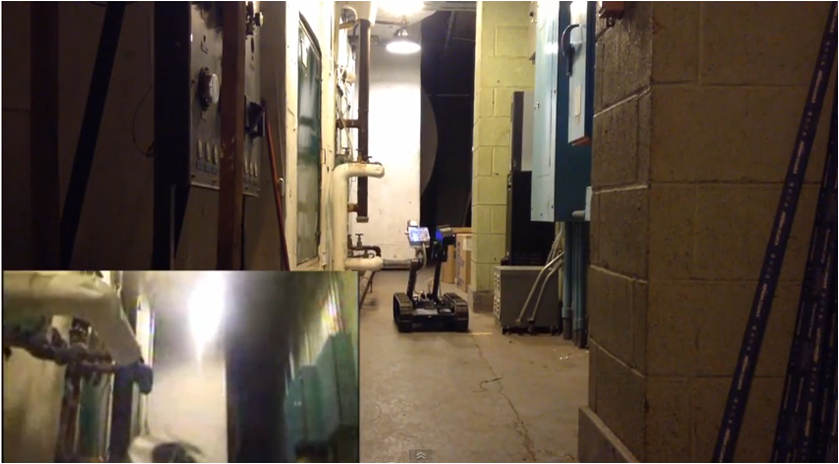
\includegraphics[width=0.48\textwidth]{./pictures/concept}
	\caption{ARIBO-IH prototype vehicle inspecting a gas leak in a notional hazardous site. The inset in the lower left shows the camera view from the perspective of the robot.}
	\label{fig:concept}
\end{figure}

\subsection{Problems}

An Industrial Hygiene mission is to reduce soldier and employee exposure to environmental factors and stresses including:  chemical (e.g., liquid, particulate dust, fumes, mist, vapor and gas), physical (e.g., electromagnetic radiation, temperature, ambient pressure, noise, vibration and ionizing radiation), and biological (e.g., agents of infectious diseases, insects, mites, molds, yeasts, fungi, bacteria and viruses) elements. The majority of hazards come from industrial processes on Army installations. Army industrial hygiene personnel are at risk from exposure to these hazardous environments in the conduct of their duties. Additionally, rapidly equipping human teams for response to incidents and post-action decontamination pose difficult challenges.  

\subsection{Benefits}

Through the use of robotic-enabled ground vehicles in a structured, controlled environment, the ARIBO-IH pilot will increase researchers’, manufacturers’, and users’ understanding and familiarity of these systems in real-world operational scenarios. The ARIBO-IH pilot safely provides the service of IH inspections, removing the human IH professional from a potentially hazardous situation while reducing cost. Additionally, the project will facilitate the design, standardization, deployment, and supervision of the resulting ARIBO-IH inspection robots. Pilot locations include Fort Bragg, North Carolina and the the United States Military Academy (USMA), at West Point.  By using cadets as researchers, they are exposed to Army technologies and systems at the beginning of their careers. The benefits of generating officers with technological backgrounds in robotics systems is paramount to achieving the DoD’s long term unmanned systems goals.

\subsection{Example Uses}
The robotic systems developed under this project could be employed in a number of situations to include:
\begin{itemize}
	\item Environmental reconnaissance in routine industrial hygiene tasks and emergency response
	\item Weather station at the emission source
	\item Ventilation duct inspection
	\item Investigate suspected terrorist devices
	\item Site abatement or mitigation projects
\end{itemize}

This paper presents a solution to the industrial hygiene problem using a small ground vehicle equipped with a sensor package. The mobility platform for the system (Fig.~\ref{fig:concept}) is detailed in Sec.~\ref{sec:platform}. To allow for unattended operation in a known environment, Sec.~\ref{sec:ui} describes the user interface to remotely monitor sensor readings and toggle between teleoperation and autonomous modes. Sec.~\ref{sec:sensors} describes the sensor package used to perform the IH mission with sensor testing and results found in Sec.~\ref{sec:results}. Navigation and path planning are described in Sec.~\ref{sec:navigation}.